% Options for packages loaded elsewhere
\PassOptionsToPackage{unicode}{hyperref}
\PassOptionsToPackage{hyphens}{url}
\PassOptionsToPackage{dvipsnames,svgnames,x11names}{xcolor}
%
\documentclass[
  letterpaper,
  DIV=11,
  numbers=noendperiod]{scrartcl}

\usepackage{amsmath,amssymb}
\usepackage{iftex}
\ifPDFTeX
  \usepackage[T1]{fontenc}
  \usepackage[utf8]{inputenc}
  \usepackage{textcomp} % provide euro and other symbols
\else % if luatex or xetex
  \usepackage{unicode-math}
  \defaultfontfeatures{Scale=MatchLowercase}
  \defaultfontfeatures[\rmfamily]{Ligatures=TeX,Scale=1}
\fi
\usepackage{lmodern}
\ifPDFTeX\else  
    % xetex/luatex font selection
\fi
% Use upquote if available, for straight quotes in verbatim environments
\IfFileExists{upquote.sty}{\usepackage{upquote}}{}
\IfFileExists{microtype.sty}{% use microtype if available
  \usepackage[]{microtype}
  \UseMicrotypeSet[protrusion]{basicmath} % disable protrusion for tt fonts
}{}
\makeatletter
\@ifundefined{KOMAClassName}{% if non-KOMA class
  \IfFileExists{parskip.sty}{%
    \usepackage{parskip}
  }{% else
    \setlength{\parindent}{0pt}
    \setlength{\parskip}{6pt plus 2pt minus 1pt}}
}{% if KOMA class
  \KOMAoptions{parskip=half}}
\makeatother
\usepackage{xcolor}
\setlength{\emergencystretch}{3em} % prevent overfull lines
\setcounter{secnumdepth}{-\maxdimen} % remove section numbering
% Make \paragraph and \subparagraph free-standing
\makeatletter
\ifx\paragraph\undefined\else
  \let\oldparagraph\paragraph
  \renewcommand{\paragraph}{
    \@ifstar
      \xxxParagraphStar
      \xxxParagraphNoStar
  }
  \newcommand{\xxxParagraphStar}[1]{\oldparagraph*{#1}\mbox{}}
  \newcommand{\xxxParagraphNoStar}[1]{\oldparagraph{#1}\mbox{}}
\fi
\ifx\subparagraph\undefined\else
  \let\oldsubparagraph\subparagraph
  \renewcommand{\subparagraph}{
    \@ifstar
      \xxxSubParagraphStar
      \xxxSubParagraphNoStar
  }
  \newcommand{\xxxSubParagraphStar}[1]{\oldsubparagraph*{#1}\mbox{}}
  \newcommand{\xxxSubParagraphNoStar}[1]{\oldsubparagraph{#1}\mbox{}}
\fi
\makeatother

\usepackage{color}
\usepackage{fancyvrb}
\newcommand{\VerbBar}{|}
\newcommand{\VERB}{\Verb[commandchars=\\\{\}]}
\DefineVerbatimEnvironment{Highlighting}{Verbatim}{commandchars=\\\{\}}
% Add ',fontsize=\small' for more characters per line
\usepackage{framed}
\definecolor{shadecolor}{RGB}{241,243,245}
\newenvironment{Shaded}{\begin{snugshade}}{\end{snugshade}}
\newcommand{\AlertTok}[1]{\textcolor[rgb]{0.68,0.00,0.00}{#1}}
\newcommand{\AnnotationTok}[1]{\textcolor[rgb]{0.37,0.37,0.37}{#1}}
\newcommand{\AttributeTok}[1]{\textcolor[rgb]{0.40,0.45,0.13}{#1}}
\newcommand{\BaseNTok}[1]{\textcolor[rgb]{0.68,0.00,0.00}{#1}}
\newcommand{\BuiltInTok}[1]{\textcolor[rgb]{0.00,0.23,0.31}{#1}}
\newcommand{\CharTok}[1]{\textcolor[rgb]{0.13,0.47,0.30}{#1}}
\newcommand{\CommentTok}[1]{\textcolor[rgb]{0.37,0.37,0.37}{#1}}
\newcommand{\CommentVarTok}[1]{\textcolor[rgb]{0.37,0.37,0.37}{\textit{#1}}}
\newcommand{\ConstantTok}[1]{\textcolor[rgb]{0.56,0.35,0.01}{#1}}
\newcommand{\ControlFlowTok}[1]{\textcolor[rgb]{0.00,0.23,0.31}{\textbf{#1}}}
\newcommand{\DataTypeTok}[1]{\textcolor[rgb]{0.68,0.00,0.00}{#1}}
\newcommand{\DecValTok}[1]{\textcolor[rgb]{0.68,0.00,0.00}{#1}}
\newcommand{\DocumentationTok}[1]{\textcolor[rgb]{0.37,0.37,0.37}{\textit{#1}}}
\newcommand{\ErrorTok}[1]{\textcolor[rgb]{0.68,0.00,0.00}{#1}}
\newcommand{\ExtensionTok}[1]{\textcolor[rgb]{0.00,0.23,0.31}{#1}}
\newcommand{\FloatTok}[1]{\textcolor[rgb]{0.68,0.00,0.00}{#1}}
\newcommand{\FunctionTok}[1]{\textcolor[rgb]{0.28,0.35,0.67}{#1}}
\newcommand{\ImportTok}[1]{\textcolor[rgb]{0.00,0.46,0.62}{#1}}
\newcommand{\InformationTok}[1]{\textcolor[rgb]{0.37,0.37,0.37}{#1}}
\newcommand{\KeywordTok}[1]{\textcolor[rgb]{0.00,0.23,0.31}{\textbf{#1}}}
\newcommand{\NormalTok}[1]{\textcolor[rgb]{0.00,0.23,0.31}{#1}}
\newcommand{\OperatorTok}[1]{\textcolor[rgb]{0.37,0.37,0.37}{#1}}
\newcommand{\OtherTok}[1]{\textcolor[rgb]{0.00,0.23,0.31}{#1}}
\newcommand{\PreprocessorTok}[1]{\textcolor[rgb]{0.68,0.00,0.00}{#1}}
\newcommand{\RegionMarkerTok}[1]{\textcolor[rgb]{0.00,0.23,0.31}{#1}}
\newcommand{\SpecialCharTok}[1]{\textcolor[rgb]{0.37,0.37,0.37}{#1}}
\newcommand{\SpecialStringTok}[1]{\textcolor[rgb]{0.13,0.47,0.30}{#1}}
\newcommand{\StringTok}[1]{\textcolor[rgb]{0.13,0.47,0.30}{#1}}
\newcommand{\VariableTok}[1]{\textcolor[rgb]{0.07,0.07,0.07}{#1}}
\newcommand{\VerbatimStringTok}[1]{\textcolor[rgb]{0.13,0.47,0.30}{#1}}
\newcommand{\WarningTok}[1]{\textcolor[rgb]{0.37,0.37,0.37}{\textit{#1}}}

\providecommand{\tightlist}{%
  \setlength{\itemsep}{0pt}\setlength{\parskip}{0pt}}\usepackage{longtable,booktabs,array}
\usepackage{calc} % for calculating minipage widths
% Correct order of tables after \paragraph or \subparagraph
\usepackage{etoolbox}
\makeatletter
\patchcmd\longtable{\par}{\if@noskipsec\mbox{}\fi\par}{}{}
\makeatother
% Allow footnotes in longtable head/foot
\IfFileExists{footnotehyper.sty}{\usepackage{footnotehyper}}{\usepackage{footnote}}
\makesavenoteenv{longtable}
\usepackage{graphicx}
\makeatletter
\def\maxwidth{\ifdim\Gin@nat@width>\linewidth\linewidth\else\Gin@nat@width\fi}
\def\maxheight{\ifdim\Gin@nat@height>\textheight\textheight\else\Gin@nat@height\fi}
\makeatother
% Scale images if necessary, so that they will not overflow the page
% margins by default, and it is still possible to overwrite the defaults
% using explicit options in \includegraphics[width, height, ...]{}
\setkeys{Gin}{width=\maxwidth,height=\maxheight,keepaspectratio}
% Set default figure placement to htbp
\makeatletter
\def\fps@figure{htbp}
\makeatother

\usepackage{booktabs}
\usepackage{longtable}
\usepackage{array}
\usepackage{multirow}
\usepackage{wrapfig}
\usepackage{float}
\usepackage{colortbl}
\usepackage{pdflscape}
\usepackage{tabu}
\usepackage{threeparttable}
\usepackage{threeparttablex}
\usepackage[normalem]{ulem}
\usepackage{makecell}
\usepackage{xcolor}
\KOMAoption{captions}{tableheading}
\makeatletter
\@ifpackageloaded{caption}{}{\usepackage{caption}}
\AtBeginDocument{%
\ifdefined\contentsname
  \renewcommand*\contentsname{Table of contents}
\else
  \newcommand\contentsname{Table of contents}
\fi
\ifdefined\listfigurename
  \renewcommand*\listfigurename{List of Figures}
\else
  \newcommand\listfigurename{List of Figures}
\fi
\ifdefined\listtablename
  \renewcommand*\listtablename{List of Tables}
\else
  \newcommand\listtablename{List of Tables}
\fi
\ifdefined\figurename
  \renewcommand*\figurename{Figure}
\else
  \newcommand\figurename{Figure}
\fi
\ifdefined\tablename
  \renewcommand*\tablename{Table}
\else
  \newcommand\tablename{Table}
\fi
}
\@ifpackageloaded{float}{}{\usepackage{float}}
\floatstyle{ruled}
\@ifundefined{c@chapter}{\newfloat{codelisting}{h}{lop}}{\newfloat{codelisting}{h}{lop}[chapter]}
\floatname{codelisting}{Listing}
\newcommand*\listoflistings{\listof{codelisting}{List of Listings}}
\makeatother
\makeatletter
\makeatother
\makeatletter
\@ifpackageloaded{caption}{}{\usepackage{caption}}
\@ifpackageloaded{subcaption}{}{\usepackage{subcaption}}
\makeatother
\ifLuaTeX
  \usepackage{selnolig}  % disable illegal ligatures
\fi
\usepackage{bookmark}

\IfFileExists{xurl.sty}{\usepackage{xurl}}{} % add URL line breaks if available
\urlstyle{same} % disable monospaced font for URLs
\hypersetup{
  colorlinks=true,
  linkcolor={blue},
  filecolor={Maroon},
  citecolor={Blue},
  urlcolor={Blue},
  pdfcreator={LaTeX via pandoc}}

\author{}
\date{}

\begin{document}

\begin{Shaded}
\begin{Highlighting}[]
\FunctionTok{library}\NormalTok{(tidyverse)}
\FunctionTok{library}\NormalTok{(cmdstanr)}
\FunctionTok{source}\NormalTok{(}\StringTok{"scripts/functions.R"}\NormalTok{)}
\NormalTok{df }\OtherTok{\textless{}{-}} \FunctionTok{read.csv}\NormalTok{(}\StringTok{"data/main.csv"}\NormalTok{)}
\FunctionTok{set.seed}\NormalTok{(}\DecValTok{12042014}\NormalTok{)}
\end{Highlighting}
\end{Shaded}

\subsubsection{The Bayesian Bootstrap}\label{the-bayesian-bootstrap}

\begin{align*}
w &\sim Dirichlet(\alpha)  \\
\mu &= \sum_{i=1}^nw_ix_i \\
\sigma &= \sqrt{\sum_{i=1}^nw_i(x_i-\sum_{i=1}^nw_ix_i)^2}
\end{align*}

\subsubsection{Posterior Predictive
Checks}\label{posterior-predictive-checks}

\paragraph{1DAG}\label{dag}

\begin{Shaded}
\begin{Highlighting}[]
\FunctionTok{post\_pred\_check}\NormalTok{(df, }\StringTok{"day\_4"}\NormalTok{, }\AttributeTok{lik =} \StringTok{"normal"}\NormalTok{)}
\end{Highlighting}
\end{Shaded}

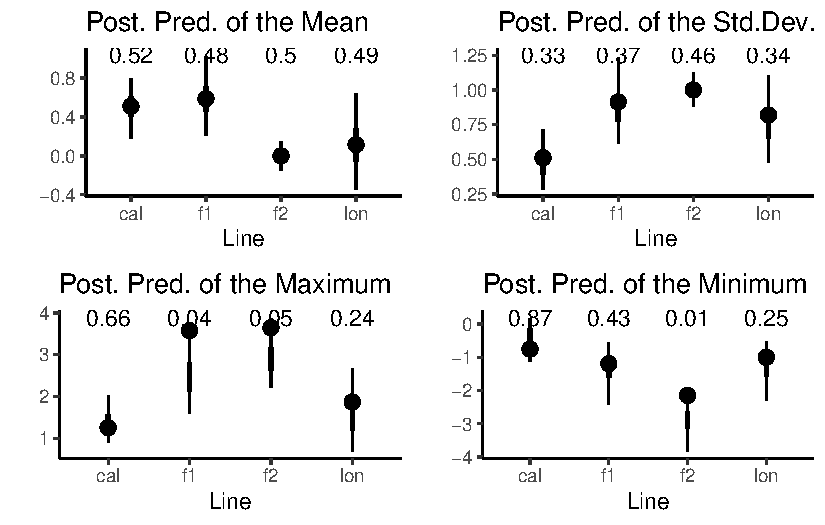
\includegraphics{analysis_files/figure-pdf/unnamed-chunk-2-1.pdf}

\begin{Shaded}
\begin{Highlighting}[]
\CommentTok{\# post\_pred\_check(df, "day\_4", lik = "gamma")}
\CommentTok{\# post\_pred\_check(df, "day\_4", lik = "log{-}normal")}
\end{Highlighting}
\end{Shaded}

\paragraph{14DAG}\label{dag-1}

\begin{Shaded}
\begin{Highlighting}[]
\FunctionTok{post\_pred\_check}\NormalTok{(df, }\StringTok{"day\_17"}\NormalTok{, }\StringTok{"normal"}\NormalTok{)}
\end{Highlighting}
\end{Shaded}

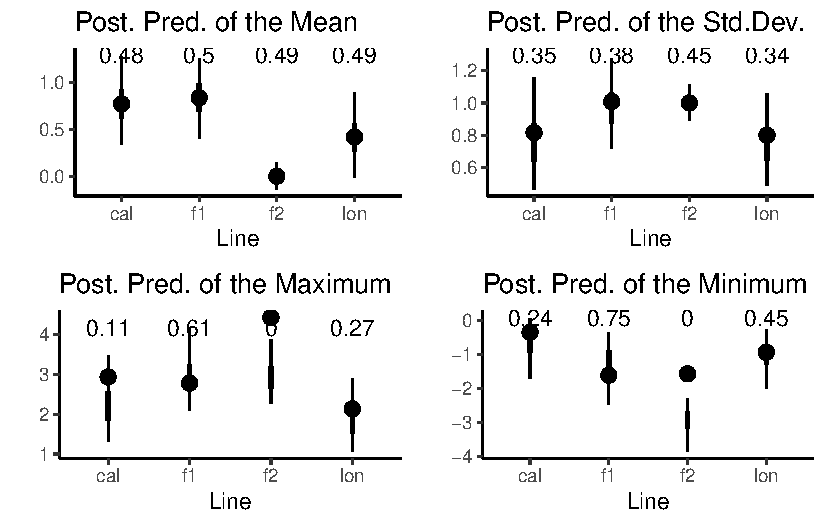
\includegraphics{analysis_files/figure-pdf/unnamed-chunk-3-1.pdf}

\begin{Shaded}
\begin{Highlighting}[]
\CommentTok{\# post\_pred\_check(df, "day\_17", "gamma")}
\CommentTok{\# post\_pred\_check(df, "day\_17", "log{-}normal")}
\end{Highlighting}
\end{Shaded}

\paragraph{RGR}\label{rgr}

\begin{Shaded}
\begin{Highlighting}[]
\FunctionTok{post\_pred\_check}\NormalTok{(df, }\StringTok{"rgr"}\NormalTok{, }\StringTok{"normal"}\NormalTok{)}
\end{Highlighting}
\end{Shaded}

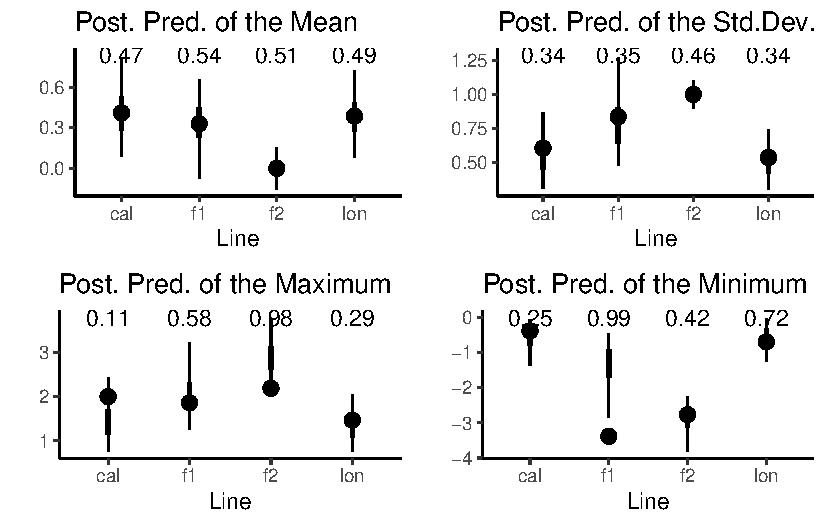
\includegraphics{analysis_files/figure-pdf/unnamed-chunk-4-1.pdf}

\begin{Shaded}
\begin{Highlighting}[]
\CommentTok{\# post\_pred\_check(df, "rgr", "gamma")}
\CommentTok{\# post\_pred\_check(df, "rgr", "log{-}normal")}
\end{Highlighting}
\end{Shaded}

\paragraph{Height}\label{height}

\begin{Shaded}
\begin{Highlighting}[]
\FunctionTok{post\_pred\_check}\NormalTok{(df, }\StringTok{"height\_122"}\NormalTok{, }\StringTok{"normal"}\NormalTok{)}
\end{Highlighting}
\end{Shaded}

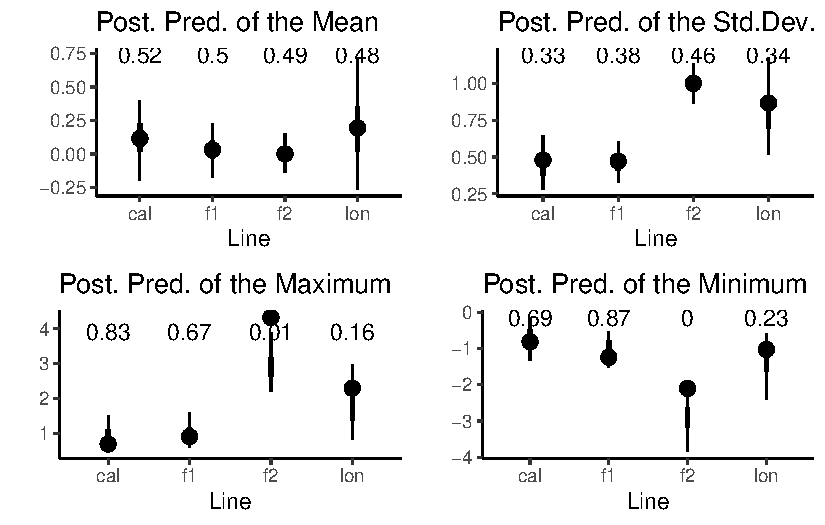
\includegraphics{analysis_files/figure-pdf/unnamed-chunk-5-1.pdf}

\begin{Shaded}
\begin{Highlighting}[]
\CommentTok{\# post\_pred\_check(df, "height\_122", "gamma")}
\CommentTok{\# post\_pred\_check(df, "height\_122", "log{-}normal")}
\end{Highlighting}
\end{Shaded}

\subsubsection{Posterior Predictive Distributions of
Delta}\label{posterior-predictive-distributions-of-delta}

\begin{Shaded}
\begin{Highlighting}[]
\NormalTok{dag1 }\OtherTok{\textless{}{-}} \FunctionTok{post\_pred}\NormalTok{(df, }\StringTok{"day\_4"}\NormalTok{, }\StringTok{"normal"}\NormalTok{)}\SpecialCharTok{$}\NormalTok{delta\_pp}
\NormalTok{dag14 }\OtherTok{\textless{}{-}} \FunctionTok{post\_pred}\NormalTok{(df, }\StringTok{"day\_17"}\NormalTok{, }\StringTok{"normal"}\NormalTok{)}\SpecialCharTok{$}\NormalTok{delta\_pp}
\NormalTok{rgr }\OtherTok{\textless{}{-}} \FunctionTok{post\_pred}\NormalTok{(df, }\StringTok{"rgr"}\NormalTok{, }\StringTok{"normal"}\NormalTok{)}\SpecialCharTok{$}\NormalTok{delta\_pp}
\NormalTok{height }\OtherTok{\textless{}{-}} \FunctionTok{post\_pred}\NormalTok{(df, }\StringTok{"height\_122"}\NormalTok{, }\StringTok{"normal"}\NormalTok{)}\SpecialCharTok{$}\NormalTok{delta\_pp}

\FunctionTok{data.frame}\NormalTok{(}\AttributeTok{DAG1 =}\NormalTok{ dag1, }\AttributeTok{DAG14=}\NormalTok{ dag14, }
           \AttributeTok{RGR =}\NormalTok{ rgr, }\AttributeTok{Height =}\NormalTok{ height) }\SpecialCharTok{\%\textgreater{}\%} 
  \FunctionTok{pivot\_longer}\NormalTok{(}\DecValTok{1}\SpecialCharTok{:}\DecValTok{4}\NormalTok{, }\AttributeTok{names\_to =} \StringTok{"trait"}\NormalTok{, }\AttributeTok{values\_to =} \StringTok{"delta"}\NormalTok{) }\SpecialCharTok{\%\textgreater{}\%} 
  \FunctionTok{mutate}\NormalTok{(}\AttributeTok{trait =} \FunctionTok{factor}\NormalTok{(trait, }\AttributeTok{levels =} \FunctionTok{c}\NormalTok{(}\StringTok{"Height"}\NormalTok{, }\StringTok{"DAG14"}\NormalTok{,}\StringTok{"DAG1"}\NormalTok{, }\StringTok{"RGR"}\NormalTok{))) }\SpecialCharTok{\%\textgreater{}\%} 
  \FunctionTok{group\_by}\NormalTok{(trait) }\SpecialCharTok{\%\textgreater{}\%} 
  \FunctionTok{summarise}\NormalTok{(}\AttributeTok{upr =} \FunctionTok{quantile}\NormalTok{(delta, .}\DecValTok{975}\NormalTok{),}
            \AttributeTok{lwr =} \FunctionTok{quantile}\NormalTok{(delta, .}\DecValTok{025}\NormalTok{),}
            \AttributeTok{upr.5 =} \FunctionTok{quantile}\NormalTok{(delta, .}\DecValTok{75}\NormalTok{),}
            \AttributeTok{lwr.5 =} \FunctionTok{quantile}\NormalTok{(delta, .}\DecValTok{25}\NormalTok{)) }\SpecialCharTok{\%\textgreater{}\%} 
  \FunctionTok{ggplot}\NormalTok{() }\SpecialCharTok{+}
  \FunctionTok{geom\_vline}\NormalTok{(}\AttributeTok{xintercept =} \DecValTok{0}\NormalTok{, }\AttributeTok{color =} \StringTok{"grey"}\NormalTok{, }\AttributeTok{linewidth =} \DecValTok{1}\NormalTok{) }\SpecialCharTok{+}
  \FunctionTok{geom\_errorbarh}\NormalTok{(}\FunctionTok{aes}\NormalTok{(}\AttributeTok{y =}\NormalTok{ trait, }\AttributeTok{xmin =}\NormalTok{ lwr, }\AttributeTok{xmax =}\NormalTok{ upr), }\AttributeTok{height =} \DecValTok{0}\NormalTok{, }
                 \AttributeTok{linewidth =} \DecValTok{1}\NormalTok{) }\SpecialCharTok{+}
  \FunctionTok{geom\_errorbarh}\NormalTok{(}\FunctionTok{aes}\NormalTok{(}\AttributeTok{y =}\NormalTok{ trait, }\AttributeTok{xmin =}\NormalTok{ lwr}\FloatTok{.5}\NormalTok{, }\AttributeTok{xmax =}\NormalTok{ upr}\FloatTok{.5}\NormalTok{), }\AttributeTok{height =} \DecValTok{0}\NormalTok{, }
                 \AttributeTok{linewidth =} \DecValTok{2}\NormalTok{) }\SpecialCharTok{+}
  \FunctionTok{theme\_minimal}\NormalTok{() }\SpecialCharTok{+}
  \FunctionTok{labs}\NormalTok{(}\AttributeTok{y =} \StringTok{"Trait"}\NormalTok{,}
       \AttributeTok{x =} \StringTok{"O(F2) {-} E(F2)"}\NormalTok{)}
\end{Highlighting}
\end{Shaded}

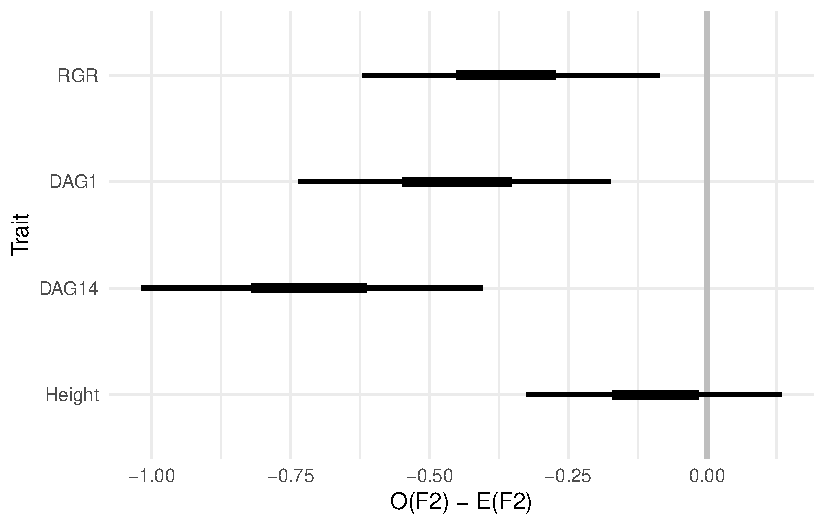
\includegraphics{analysis_files/figure-pdf/unnamed-chunk-6-1.pdf}

\subsubsection{}\label{section}

\begin{Shaded}
\begin{Highlighting}[]
\NormalTok{dag1 }\OtherTok{\textless{}{-}} \FunctionTok{post\_pred}\NormalTok{(df, }\StringTok{"day\_4"}\NormalTok{, }\StringTok{"normal"}\NormalTok{)}\SpecialCharTok{$}\NormalTok{boots}
\NormalTok{dag1 }\OtherTok{\textless{}{-}}\NormalTok{ dag1 }\SpecialCharTok{\%\textgreater{}\%} 
  \FunctionTok{pivot\_longer}\NormalTok{(}\DecValTok{1}\SpecialCharTok{:}\DecValTok{5}\NormalTok{, }\AttributeTok{names\_to =} \StringTok{"line"}\NormalTok{, }\AttributeTok{values\_to =} \StringTok{"trait"}\NormalTok{) }\SpecialCharTok{\%\textgreater{}\%} 
  \FunctionTok{group\_by}\NormalTok{(line) }\SpecialCharTok{\%\textgreater{}\%} 
  \FunctionTok{summarise}\NormalTok{(}\AttributeTok{mu =} \FunctionTok{round}\NormalTok{(}\FunctionTok{mean}\NormalTok{(trait),}\DecValTok{2}\NormalTok{),}
            \AttributeTok{upr =} \FunctionTok{round}\NormalTok{(}\FunctionTok{quantile}\NormalTok{(trait, .}\DecValTok{975}\NormalTok{),}\DecValTok{2}\NormalTok{),}
            \AttributeTok{lwr =} \FunctionTok{round}\NormalTok{(}\FunctionTok{quantile}\NormalTok{(trait, .}\DecValTok{025}\NormalTok{),}\DecValTok{2}\NormalTok{),}
            \AttributeTok{upr.5 =} \FunctionTok{round}\NormalTok{(}\FunctionTok{quantile}\NormalTok{(trait, .}\DecValTok{75}\NormalTok{),}\DecValTok{2}\NormalTok{),}
            \AttributeTok{lwr.5 =} \FunctionTok{round}\NormalTok{(}\FunctionTok{quantile}\NormalTok{(trait, .}\DecValTok{25}\NormalTok{),}\DecValTok{2}\NormalTok{)) }\SpecialCharTok{\%\textgreater{}\%} 
  \FunctionTok{mutate}\NormalTok{(}\AttributeTok{trait =} \StringTok{"1DAG"}\NormalTok{)}

\NormalTok{dag14 }\OtherTok{\textless{}{-}} \FunctionTok{post\_pred}\NormalTok{(df, }\StringTok{"day\_17"}\NormalTok{, }\StringTok{"normal"}\NormalTok{)}\SpecialCharTok{$}\NormalTok{boots}
\NormalTok{dag14 }\OtherTok{\textless{}{-}}\NormalTok{ dag14 }\SpecialCharTok{\%\textgreater{}\%} 
  \FunctionTok{pivot\_longer}\NormalTok{(}\DecValTok{1}\SpecialCharTok{:}\DecValTok{5}\NormalTok{, }\AttributeTok{names\_to =} \StringTok{"line"}\NormalTok{, }\AttributeTok{values\_to =} \StringTok{"trait"}\NormalTok{) }\SpecialCharTok{\%\textgreater{}\%} 
  \FunctionTok{group\_by}\NormalTok{(line) }\SpecialCharTok{\%\textgreater{}\%} 
  \FunctionTok{summarise}\NormalTok{(}\AttributeTok{mu =} \FunctionTok{round}\NormalTok{(}\FunctionTok{mean}\NormalTok{(trait),}\DecValTok{2}\NormalTok{),}
            \AttributeTok{upr =} \FunctionTok{round}\NormalTok{(}\FunctionTok{quantile}\NormalTok{(trait, .}\DecValTok{975}\NormalTok{),}\DecValTok{2}\NormalTok{),}
            \AttributeTok{lwr =} \FunctionTok{round}\NormalTok{(}\FunctionTok{quantile}\NormalTok{(trait, .}\DecValTok{025}\NormalTok{),}\DecValTok{2}\NormalTok{),}
            \AttributeTok{upr.5 =} \FunctionTok{round}\NormalTok{(}\FunctionTok{quantile}\NormalTok{(trait, .}\DecValTok{75}\NormalTok{),}\DecValTok{2}\NormalTok{),}
            \AttributeTok{lwr.5 =} \FunctionTok{round}\NormalTok{(}\FunctionTok{quantile}\NormalTok{(trait, .}\DecValTok{25}\NormalTok{),}\DecValTok{2}\NormalTok{)) }\SpecialCharTok{\%\textgreater{}\%} 
  \FunctionTok{mutate}\NormalTok{(}\AttributeTok{trait =} \StringTok{"14DAG"}\NormalTok{)}

\NormalTok{rgr }\OtherTok{\textless{}{-}} \FunctionTok{post\_pred}\NormalTok{(df, }\StringTok{"rgr"}\NormalTok{, }\StringTok{"normal"}\NormalTok{)}\SpecialCharTok{$}\NormalTok{boots}
\NormalTok{rgr }\OtherTok{\textless{}{-}}\NormalTok{ rgr }\SpecialCharTok{\%\textgreater{}\%} 
  \FunctionTok{pivot\_longer}\NormalTok{(}\DecValTok{1}\SpecialCharTok{:}\DecValTok{5}\NormalTok{, }\AttributeTok{names\_to =} \StringTok{"line"}\NormalTok{, }\AttributeTok{values\_to =} \StringTok{"trait"}\NormalTok{) }\SpecialCharTok{\%\textgreater{}\%} 
  \FunctionTok{group\_by}\NormalTok{(line) }\SpecialCharTok{\%\textgreater{}\%} 
  \FunctionTok{summarise}\NormalTok{(}\AttributeTok{mu =} \FunctionTok{round}\NormalTok{(}\FunctionTok{mean}\NormalTok{(trait),}\DecValTok{2}\NormalTok{),}
            \AttributeTok{upr =} \FunctionTok{round}\NormalTok{(}\FunctionTok{quantile}\NormalTok{(trait, .}\DecValTok{975}\NormalTok{),}\DecValTok{2}\NormalTok{),}
            \AttributeTok{lwr =} \FunctionTok{round}\NormalTok{(}\FunctionTok{quantile}\NormalTok{(trait, .}\DecValTok{025}\NormalTok{),}\DecValTok{2}\NormalTok{),}
            \AttributeTok{upr.5 =} \FunctionTok{round}\NormalTok{(}\FunctionTok{quantile}\NormalTok{(trait, .}\DecValTok{75}\NormalTok{),}\DecValTok{2}\NormalTok{),}
            \AttributeTok{lwr.5 =} \FunctionTok{round}\NormalTok{(}\FunctionTok{quantile}\NormalTok{(trait, .}\DecValTok{25}\NormalTok{),}\DecValTok{2}\NormalTok{)) }\SpecialCharTok{\%\textgreater{}\%} 
  \FunctionTok{mutate}\NormalTok{(}\AttributeTok{trait =} \StringTok{"RGR"}\NormalTok{)}

\NormalTok{height }\OtherTok{\textless{}{-}} \FunctionTok{post\_pred}\NormalTok{(df, }\StringTok{"height\_122"}\NormalTok{, }\StringTok{"normal"}\NormalTok{)}\SpecialCharTok{$}\NormalTok{boots}
\NormalTok{height }\OtherTok{\textless{}{-}}\NormalTok{ height }\SpecialCharTok{\%\textgreater{}\%} 
  \FunctionTok{pivot\_longer}\NormalTok{(}\DecValTok{1}\SpecialCharTok{:}\DecValTok{5}\NormalTok{, }\AttributeTok{names\_to =} \StringTok{"line"}\NormalTok{, }\AttributeTok{values\_to =} \StringTok{"trait"}\NormalTok{) }\SpecialCharTok{\%\textgreater{}\%} 
  \FunctionTok{group\_by}\NormalTok{(line) }\SpecialCharTok{\%\textgreater{}\%} 
  \FunctionTok{summarise}\NormalTok{(}\AttributeTok{mu =} \FunctionTok{round}\NormalTok{(}\FunctionTok{mean}\NormalTok{(trait),}\DecValTok{2}\NormalTok{),}
            \AttributeTok{upr =} \FunctionTok{round}\NormalTok{(}\FunctionTok{quantile}\NormalTok{(trait, .}\DecValTok{975}\NormalTok{),}\DecValTok{2}\NormalTok{),}
            \AttributeTok{lwr =} \FunctionTok{round}\NormalTok{(}\FunctionTok{quantile}\NormalTok{(trait, .}\DecValTok{025}\NormalTok{),}\DecValTok{2}\NormalTok{),}
            \AttributeTok{upr.5 =} \FunctionTok{round}\NormalTok{(}\FunctionTok{quantile}\NormalTok{(trait, .}\DecValTok{75}\NormalTok{),}\DecValTok{2}\NormalTok{),}
            \AttributeTok{lwr.5 =} \FunctionTok{round}\NormalTok{(}\FunctionTok{quantile}\NormalTok{(trait, .}\DecValTok{25}\NormalTok{),}\DecValTok{2}\NormalTok{)) }\SpecialCharTok{\%\textgreater{}\%} 
  \FunctionTok{mutate}\NormalTok{(}\AttributeTok{trait =} \StringTok{"Height"}\NormalTok{)}

\FunctionTok{library}\NormalTok{(knitr)}
\FunctionTok{library}\NormalTok{(kableExtra)}
\end{Highlighting}
\end{Shaded}

\begin{verbatim}

Attaching package: 'kableExtra'
\end{verbatim}

\begin{verbatim}
The following object is masked from 'package:dplyr':

    group_rows
\end{verbatim}

\begin{Shaded}
\begin{Highlighting}[]
\NormalTok{tab\_dat }\OtherTok{\textless{}{-}} \FunctionTok{bind\_rows}\NormalTok{(dag1, dag14, rgr, height)}

\NormalTok{tab\_dat }\SpecialCharTok{\%\textgreater{}\%} 
  \FunctionTok{select}\NormalTok{(}\AttributeTok{Line =}\NormalTok{ line, }\AttributeTok{Mean =}\NormalTok{ mu, }\StringTok{"2.5\%"} \OtherTok{=}\NormalTok{ lwr, }\StringTok{"25\%"} \OtherTok{=}\NormalTok{ lwr}\FloatTok{.5}\NormalTok{,}
         \StringTok{"75\%"} \OtherTok{=}\NormalTok{ upr}\FloatTok{.5}\NormalTok{, }\StringTok{"97.5\%"} \OtherTok{=}\NormalTok{ upr) }\SpecialCharTok{\%\textgreater{}\%} 
  \FunctionTok{mutate}\NormalTok{(}\AttributeTok{Line =} \FunctionTok{case\_when}\NormalTok{(Line }\SpecialCharTok{==} \StringTok{"cal"} \SpecialCharTok{\textasciitilde{}} \StringTok{"Calycinus"}\NormalTok{,}
\NormalTok{                          Line }\SpecialCharTok{==} \StringTok{"f1"} \SpecialCharTok{\textasciitilde{}} \StringTok{"F1"}\NormalTok{,}
\NormalTok{                          Line }\SpecialCharTok{==} \StringTok{"f2"} \SpecialCharTok{\textasciitilde{}} \StringTok{"F2"}\NormalTok{,}
\NormalTok{                          Line }\SpecialCharTok{==} \StringTok{"lon"} \SpecialCharTok{\textasciitilde{}} \StringTok{"Longiflorus"}\NormalTok{,}
\NormalTok{                          Line }\SpecialCharTok{==} \StringTok{"e\_f2"} \SpecialCharTok{\textasciitilde{}} \StringTok{"Expected F2"}\NormalTok{)) }\SpecialCharTok{\%\textgreater{}\%} 
  \FunctionTok{kbl}\NormalTok{() }\SpecialCharTok{\%\textgreater{}\%} 
  \FunctionTok{kable\_classic\_2}\NormalTok{() }\SpecialCharTok{\%\textgreater{}\%} 
  \FunctionTok{add\_header\_above}\NormalTok{(}\FunctionTok{c}\NormalTok{(}\StringTok{" "} \OtherTok{=} \DecValTok{1}\NormalTok{, }\StringTok{"Posterior Distribution of Line Mean"} \OtherTok{=} \DecValTok{5}\NormalTok{)) }\SpecialCharTok{\%\textgreater{}\%}
  \FunctionTok{pack\_rows}\NormalTok{(}\StringTok{"1DAG"}\NormalTok{,}\DecValTok{1}\NormalTok{,}\DecValTok{5}\NormalTok{) }\SpecialCharTok{\%\textgreater{}\%}
  \FunctionTok{pack\_rows}\NormalTok{(}\StringTok{"14DAG"}\NormalTok{,}\DecValTok{6}\NormalTok{,}\DecValTok{10}\NormalTok{) }\SpecialCharTok{\%\textgreater{}\%}
  \FunctionTok{pack\_rows}\NormalTok{(}\StringTok{"RGR"}\NormalTok{, }\DecValTok{11}\NormalTok{,}\DecValTok{15}\NormalTok{) }\SpecialCharTok{\%\textgreater{}\%}
  \FunctionTok{pack\_rows}\NormalTok{(}\StringTok{"Height"}\NormalTok{,}\DecValTok{16}\NormalTok{,}\DecValTok{20}\NormalTok{)}
\end{Highlighting}
\end{Shaded}

\begin{table}
\centering
\begin{tabular}[t]{l|r|r|r|r|r}
\hline
\multicolumn{1}{c|}{ } & \multicolumn{5}{c}{Posterior Distribution of Line Mean} \\
\cline{2-6}
Line & Mean & 2.5\% & 25\% & 75\% & 97.5\%\\
\hline
\multicolumn{6}{l}{\textbf{1DAG}}\\
\hline
\hspace{1em}Calycinus & 0.51 & 0.28 & 0.44 & 0.58 & 0.72\\
\hline
\hspace{1em}Expected F2 & 0.45 & 0.28 & 0.39 & 0.51 & 0.63\\
\hline
\hspace{1em}F1 & 0.59 & 0.33 & 0.49 & 0.68 & 0.88\\
\hline
\hspace{1em}F2 & 0.00 & -0.10 & -0.04 & 0.04 & 0.11\\
\hline
\hspace{1em}Longiflorus & 0.12 & -0.21 & -0.01 & 0.23 & 0.48\\
\hline
\multicolumn{6}{l}{\textbf{14DAG}}\\
\hline
\hspace{1em}Calycinus & 0.77 & 0.47 & 0.65 & 0.88 & 1.13\\
\hline
\hspace{1em}Expected F2 & 0.72 & 0.53 & 0.65 & 0.78 & 0.91\\
\hline
\hspace{1em}F1 & 0.84 & 0.53 & 0.74 & 0.95 & 1.13\\
\hline
\hspace{1em}F2 & 0.00 & -0.10 & -0.03 & 0.03 & 0.10\\
\hline
\hspace{1em}Longiflorus & 0.42 & 0.11 & 0.31 & 0.52 & 0.75\\
\hline
\multicolumn{6}{l}{\textbf{RGR}}\\
\hline
\hspace{1em}Calycinus & 0.41 & 0.19 & 0.32 & 0.49 & 0.70\\
\hline
\hspace{1em}Expected F2 & 0.36 & 0.20 & 0.31 & 0.42 & 0.51\\
\hline
\hspace{1em}F1 & 0.33 & 0.04 & 0.26 & 0.42 & 0.55\\
\hline
\hspace{1em}F2 & 0.00 & -0.11 & -0.04 & 0.04 & 0.11\\
\hline
\hspace{1em}Longiflorus & 0.38 & 0.16 & 0.30 & 0.46 & 0.62\\
\hline
\multicolumn{6}{l}{\textbf{Height}}\\
\hline
\hspace{1em}Calycinus & 0.11 & -0.11 & 0.04 & 0.19 & 0.32\\
\hline
\hspace{1em}Expected F2 & 0.09 & -0.03 & 0.05 & 0.13 & 0.22\\
\hline
\hspace{1em}F1 & 0.03 & -0.11 & -0.02 & 0.08 & 0.17\\
\hline
\hspace{1em}F2 & 0.00 & -0.10 & -0.04 & 0.03 & 0.11\\
\hline
\hspace{1em}Longiflorus & 0.19 & -0.13 & 0.07 & 0.31 & 0.57\\
\hline
\end{tabular}
\end{table}

\begin{Shaded}
\begin{Highlighting}[]
\NormalTok{(p1 }\OtherTok{\textless{}{-}}\NormalTok{ dag1 }\SpecialCharTok{\%\textgreater{}\%} 
  \FunctionTok{mutate}\NormalTok{(}\AttributeTok{plon =} \FunctionTok{c}\NormalTok{(}\DecValTok{0}\NormalTok{, .}\DecValTok{51}\NormalTok{, .}\DecValTok{49}\NormalTok{, .}\DecValTok{5}\NormalTok{, }\DecValTok{1}\NormalTok{),}
         \AttributeTok{group =} \FunctionTok{c}\NormalTok{(}\StringTok{"a"}\NormalTok{, letters[}\DecValTok{2}\SpecialCharTok{:}\DecValTok{4}\NormalTok{], }\StringTok{"a"}\NormalTok{)) }\SpecialCharTok{\%\textgreater{}\%} 
  \FunctionTok{ggplot}\NormalTok{(}\FunctionTok{aes}\NormalTok{(}\AttributeTok{x =}\NormalTok{ plon, }\AttributeTok{y =}\NormalTok{ mu, }\AttributeTok{group =}\NormalTok{ group, }\AttributeTok{color =}\NormalTok{ line)) }\SpecialCharTok{+}
  \FunctionTok{geom\_line}\NormalTok{() }\SpecialCharTok{+}
  \FunctionTok{geom\_errorbar}\NormalTok{(}\FunctionTok{aes}\NormalTok{(}\AttributeTok{x =}\NormalTok{ plon, }\AttributeTok{ymax =}\NormalTok{ upr, }\AttributeTok{ymin =}\NormalTok{ lwr), }\AttributeTok{width =} \DecValTok{0}\NormalTok{, }
                \AttributeTok{linewidth =} \DecValTok{1}\NormalTok{) }\SpecialCharTok{+}
  \FunctionTok{geom\_errorbar}\NormalTok{(}\FunctionTok{aes}\NormalTok{(}\AttributeTok{x =}\NormalTok{ plon, }\AttributeTok{ymax =}\NormalTok{ upr}\FloatTok{.5}\NormalTok{, }\AttributeTok{ymin =}\NormalTok{ lwr}\FloatTok{.5}\NormalTok{), }\AttributeTok{width =} \DecValTok{0}\NormalTok{,}
                \AttributeTok{linewidth =} \DecValTok{2}\NormalTok{) }\SpecialCharTok{+}
  \FunctionTok{scale\_color\_manual}\NormalTok{(}\AttributeTok{values =} \FunctionTok{c}\NormalTok{(}\StringTok{"black"}\NormalTok{, }\StringTok{"red"}\NormalTok{, }\StringTok{"black"}\NormalTok{, }\StringTok{"blue"}\NormalTok{, }\StringTok{"black"}\NormalTok{)) }\SpecialCharTok{+}
  \FunctionTok{theme\_minimal}\NormalTok{() }\SpecialCharTok{+}
  \FunctionTok{labs}\NormalTok{(}\AttributeTok{x =} \StringTok{"Proportion Longiflorus"}\NormalTok{))}
\end{Highlighting}
\end{Shaded}

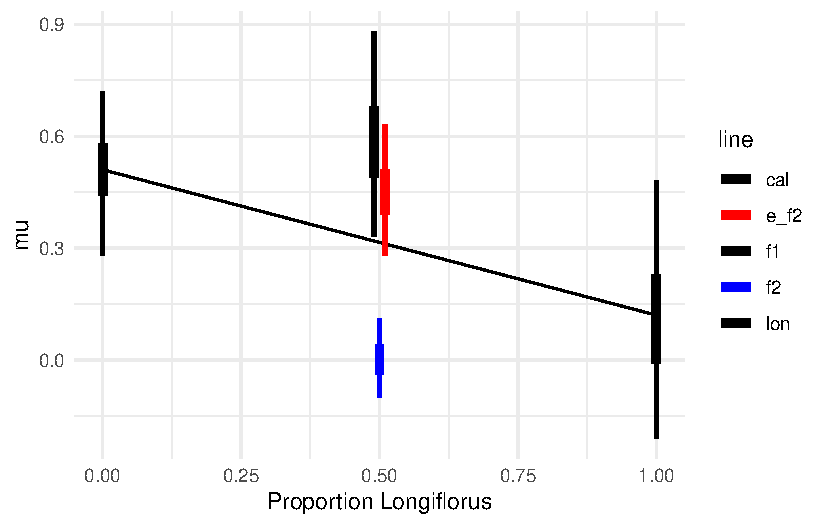
\includegraphics{analysis_files/figure-pdf/unnamed-chunk-8-1.pdf}

\[
\begin{align*}
log(size) &\sim Gamma(\alpha, \beta)\\
\alpha &= \frac{\mu^2}{\sigma^2}\\
\beta &= \frac{\mu}{\sigma^2} \\
\mu &= \alpha_{rgr} + rgr\times age\\
\sigma^2 &\sim Normal^+(0, .5)\\
\end{align*}
\]

\begin{Shaded}
\begin{Highlighting}[]
\NormalTok{d }\OtherTok{\textless{}{-}} \FunctionTok{read.csv}\NormalTok{(}\StringTok{"data/seed\_growth\_vs\_seed\_size.csv"}\NormalTok{)}


\NormalTok{rgr\_dat }\OtherTok{\textless{}{-}}\NormalTok{ d }\SpecialCharTok{\%\textgreater{}\%} 
  \FunctionTok{drop\_na}\NormalTok{(germ\_day, death\_day) }\SpecialCharTok{\%\textgreater{}\%} 
  \FunctionTok{mutate}\NormalTok{(}\AttributeTok{ind =} \DecValTok{1}\SpecialCharTok{:}\DecValTok{105}\NormalTok{) }\SpecialCharTok{\%\textgreater{}\%} 
  \FunctionTok{pivot\_longer}\NormalTok{(}\DecValTok{4}\SpecialCharTok{:}\DecValTok{10}\NormalTok{, }\AttributeTok{names\_to =} \StringTok{"day"}\NormalTok{, }\AttributeTok{values\_to =} \StringTok{"size"}\NormalTok{) }\SpecialCharTok{\%\textgreater{}\%} 
  \FunctionTok{drop\_na}\NormalTok{(size) }\SpecialCharTok{\%\textgreater{}\%} 
  \FunctionTok{mutate}\NormalTok{(}\AttributeTok{l\_size =} \FunctionTok{log}\NormalTok{(size)) }\SpecialCharTok{\%\textgreater{}\%} 
  \FunctionTok{separate}\NormalTok{(day, }\AttributeTok{into =}\NormalTok{ (}\FunctionTok{c}\NormalTok{(}\StringTok{"a"}\NormalTok{, }\StringTok{"day"}\NormalTok{))) }\SpecialCharTok{\%\textgreater{}\%} 
  \FunctionTok{mutate}\NormalTok{(}\AttributeTok{day =} \FunctionTok{as.numeric}\NormalTok{(day),}
         \AttributeTok{age =}\NormalTok{ day }\SpecialCharTok{{-}}\NormalTok{ germ\_day) }\SpecialCharTok{\%\textgreater{}\%} 
  \FunctionTok{filter}\NormalTok{(age }\SpecialCharTok{\textgreater{}} \DecValTok{0}\NormalTok{) }\SpecialCharTok{\%\textgreater{}\%} 
  \FunctionTok{select}\NormalTok{(ind, age, l\_size)}

\NormalTok{full }\OtherTok{\textless{}{-}}\NormalTok{ d }\SpecialCharTok{\%\textgreater{}\%} \FunctionTok{drop\_na}\NormalTok{(germ\_day, death\_day) }\SpecialCharTok{\%\textgreater{}\%}
  \FunctionTok{mutate}\NormalTok{(}\AttributeTok{ind =} \DecValTok{1}\SpecialCharTok{:}\DecValTok{105}\NormalTok{) }\SpecialCharTok{\%\textgreater{}\%} 
  \FunctionTok{pivot\_longer}\NormalTok{(}\DecValTok{4}\SpecialCharTok{:}\DecValTok{10}\NormalTok{, }\AttributeTok{names\_to =} \StringTok{"day"}\NormalTok{, }\AttributeTok{values\_to =} \StringTok{"size"}\NormalTok{) }\SpecialCharTok{\%\textgreater{}\%} 
  \FunctionTok{drop\_na}\NormalTok{(size) }\SpecialCharTok{\%\textgreater{}\%}
  \FunctionTok{drop\_na}\NormalTok{(size) }\SpecialCharTok{\%\textgreater{}\%} 
  \FunctionTok{separate}\NormalTok{(day, }\FunctionTok{c}\NormalTok{(}\StringTok{"fubar"}\NormalTok{, }\StringTok{"day"}\NormalTok{)) }\SpecialCharTok{\%\textgreater{}\%} 
  \FunctionTok{mutate}\NormalTok{(}\AttributeTok{day =} \FunctionTok{as.numeric}\NormalTok{(day)) }\SpecialCharTok{\%\textgreater{}\%} 
  \FunctionTok{select}\NormalTok{(ind, seed\_size, germ\_day, death\_day, day, size) }\SpecialCharTok{\%\textgreater{}\%} 
  \FunctionTok{mutate}\NormalTok{(}\AttributeTok{age =}\NormalTok{ day }\SpecialCharTok{{-}}\NormalTok{ germ\_day) }\SpecialCharTok{\%\textgreater{}\%}
  \FunctionTok{filter}\NormalTok{(age }\SpecialCharTok{==} \DecValTok{1} \SpecialCharTok{|}\NormalTok{ day }\SpecialCharTok{==} \DecValTok{17}\NormalTok{) }\SpecialCharTok{\%\textgreater{}\%}
  \FunctionTok{mutate}\NormalTok{(}\AttributeTok{tp =} \FunctionTok{ifelse}\NormalTok{(age }\SpecialCharTok{==} \DecValTok{1}\NormalTok{, }\StringTok{"start"}\NormalTok{,}\StringTok{"finish"}\NormalTok{)) }\SpecialCharTok{\%\textgreater{}\%} 
  \FunctionTok{pivot\_wider}\NormalTok{(}\AttributeTok{id\_cols =} \FunctionTok{c}\NormalTok{(ind, seed\_size, germ\_day, death\_day),}
              \AttributeTok{names\_from =}\NormalTok{ tp, }\AttributeTok{values\_from =}\NormalTok{ size)}

\NormalTok{mu }\OtherTok{\textless{}{-}} \FunctionTok{mean}\NormalTok{(full}\SpecialCharTok{$}\NormalTok{start[}\SpecialCharTok{!}\NormalTok{(}\FunctionTok{is.na}\NormalTok{(full}\SpecialCharTok{$}\NormalTok{start))])}

\NormalTok{sd }\OtherTok{\textless{}{-}} \FunctionTok{sd}\NormalTok{(full}\SpecialCharTok{$}\NormalTok{start[}\SpecialCharTok{!}\NormalTok{(}\FunctionTok{is.na}\NormalTok{(full}\SpecialCharTok{$}\NormalTok{start))])}

\NormalTok{full}\SpecialCharTok{$}\NormalTok{start }\OtherTok{\textless{}{-}} \FunctionTok{ifelse}\NormalTok{(}\FunctionTok{is.na}\NormalTok{(full}\SpecialCharTok{$}\NormalTok{start), }\SpecialCharTok{{-}}\DecValTok{100}\NormalTok{, (full}\SpecialCharTok{$}\NormalTok{start }\SpecialCharTok{{-}}\NormalTok{ mu)}\SpecialCharTok{/}\NormalTok{sd)}
\NormalTok{full}\SpecialCharTok{$}\NormalTok{finish }\OtherTok{\textless{}{-}} \FunctionTok{stn}\NormalTok{(full}\SpecialCharTok{$}\NormalTok{finish)}
\NormalTok{full}\SpecialCharTok{$}\NormalTok{seed\_size }\OtherTok{\textless{}{-}} \FunctionTok{stn}\NormalTok{(full}\SpecialCharTok{$}\NormalTok{seed\_size)}
\NormalTok{full}\SpecialCharTok{$}\NormalTok{survive }\OtherTok{\textless{}{-}}\NormalTok{ full}\SpecialCharTok{$}\NormalTok{death\_day }\SpecialCharTok{{-}} \DecValTok{3}



\NormalTok{stan\_dat }\OtherTok{\textless{}{-}} \FunctionTok{list}\NormalTok{(}
  \AttributeTok{N =} \FunctionTok{nrow}\NormalTok{(full),}
  \AttributeTok{N\_tilde =} \DecValTok{200}\NormalTok{,}
  \AttributeTok{N\_obs =} \FunctionTok{sum}\NormalTok{(full}\SpecialCharTok{$}\NormalTok{start }\SpecialCharTok{!=} \SpecialCharTok{{-}}\DecValTok{100}\NormalTok{),}
  \AttributeTok{N\_miss =} \FunctionTok{sum}\NormalTok{(full}\SpecialCharTok{$}\NormalTok{start }\SpecialCharTok{==} \SpecialCharTok{{-}}\DecValTok{100}\NormalTok{),}
  \AttributeTok{ind =}\NormalTok{ full}\SpecialCharTok{$}\NormalTok{ind,}
  \AttributeTok{ii\_obs =}\NormalTok{ full}\SpecialCharTok{$}\NormalTok{ind[full}\SpecialCharTok{$}\NormalTok{start }\SpecialCharTok{!=} \SpecialCharTok{{-}}\DecValTok{100}\NormalTok{],}
  \AttributeTok{ii\_miss =}\NormalTok{ full}\SpecialCharTok{$}\NormalTok{ind[full}\SpecialCharTok{$}\NormalTok{start }\SpecialCharTok{==} \SpecialCharTok{{-}}\DecValTok{100}\NormalTok{],}
  \AttributeTok{start\_obs =}\NormalTok{ full}\SpecialCharTok{$}\NormalTok{start[full}\SpecialCharTok{$}\NormalTok{start}\SpecialCharTok{!={-}}\DecValTok{100}\NormalTok{],}
  \AttributeTok{size\_end =}\NormalTok{ full}\SpecialCharTok{$}\NormalTok{finish,}
  \AttributeTok{seed\_size =}\NormalTok{ full}\SpecialCharTok{$}\NormalTok{seed\_size,}
  \AttributeTok{germ\_day =}\NormalTok{ full}\SpecialCharTok{$}\NormalTok{germ\_day,}
  \AttributeTok{N\_rgr =} \FunctionTok{nrow}\NormalTok{(rgr\_dat),}
  \AttributeTok{l\_size =}\NormalTok{ rgr\_dat}\SpecialCharTok{$}\NormalTok{l\_size,}
  \AttributeTok{age =}\NormalTok{ rgr\_dat}\SpecialCharTok{$}\NormalTok{age,}
  \AttributeTok{ind\_rgr =}\NormalTok{ rgr\_dat}\SpecialCharTok{$}\NormalTok{ind,}
  \AttributeTok{survive =}\NormalTok{ full}\SpecialCharTok{$}\NormalTok{survive,}
  \AttributeTok{x\_tilde =} \FunctionTok{seq}\NormalTok{(}\SpecialCharTok{{-}}\DecValTok{3}\NormalTok{,}\DecValTok{3}\NormalTok{, }\AttributeTok{l =} \DecValTok{200}\NormalTok{)}
\NormalTok{)}




\NormalTok{mod }\OtherTok{\textless{}{-}} \FunctionTok{cmdstan\_model}\NormalTok{(}\StringTok{"scripts/size.stan"}\NormalTok{)}


\NormalTok{fit }\OtherTok{\textless{}{-}}\NormalTok{ mod}\SpecialCharTok{$}\FunctionTok{sample}\NormalTok{(}
  \AttributeTok{data =}\NormalTok{ stan\_dat,}
  \AttributeTok{chains =} \DecValTok{4}\NormalTok{,}
  \AttributeTok{parallel\_chains =} \DecValTok{4}\NormalTok{,}
  \AttributeTok{show\_messages =}\NormalTok{ F}
\NormalTok{)}


\NormalTok{beta\_surv }\OtherTok{\textless{}{-}}\NormalTok{ fit}\SpecialCharTok{$}\FunctionTok{draws}\NormalTok{(}\StringTok{"beta\_surv"}\NormalTok{, }\AttributeTok{format =} \StringTok{"df"}\NormalTok{)}\SpecialCharTok{$}\NormalTok{beta\_surv}
\FunctionTok{hist}\NormalTok{(beta\_surv)}
\FunctionTok{abline}\NormalTok{(}\AttributeTok{v =} \FunctionTok{quantile}\NormalTok{(beta\_surv, }\FunctionTok{c}\NormalTok{(.}\DecValTok{025}\NormalTok{, .}\DecValTok{975}\NormalTok{)), }\AttributeTok{col =} \StringTok{"red"}\NormalTok{, }\AttributeTok{lwd =} \DecValTok{3}\NormalTok{)}
\end{Highlighting}
\end{Shaded}

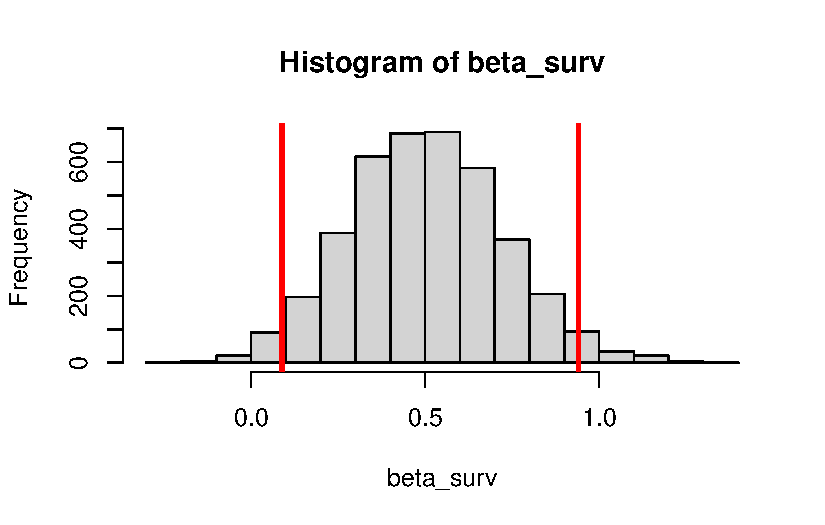
\includegraphics{analysis_files/figure-pdf/unnamed-chunk-9-1.pdf}

\begin{Shaded}
\begin{Highlighting}[]
\NormalTok{p }\OtherTok{\textless{}{-}}\NormalTok{ fit}\SpecialCharTok{$}\FunctionTok{draws}\NormalTok{(}\StringTok{"p\_tilde"}\NormalTok{, }\AttributeTok{format =} \StringTok{"df"}\NormalTok{)[,}\DecValTok{1}\SpecialCharTok{:}\DecValTok{200}\NormalTok{]}


\NormalTok{mu }\OtherTok{\textless{}{-}} \FunctionTok{apply}\NormalTok{(p, }\DecValTok{2}\NormalTok{, mean)}
\NormalTok{upr }\OtherTok{\textless{}{-}} \FunctionTok{apply}\NormalTok{(p, }\DecValTok{2}\NormalTok{, quantile, .}\DecValTok{975}\NormalTok{)}
\NormalTok{lwr }\OtherTok{\textless{}{-}} \FunctionTok{apply}\NormalTok{(p, }\DecValTok{2}\NormalTok{, quantile, .}\DecValTok{025}\NormalTok{)}
\NormalTok{upr}\FloatTok{.5} \OtherTok{\textless{}{-}} \FunctionTok{apply}\NormalTok{(p,}\DecValTok{2}\NormalTok{,quantile, .}\DecValTok{75}\NormalTok{)}
\NormalTok{lwr}\FloatTok{.5} \OtherTok{\textless{}{-}} \FunctionTok{apply}\NormalTok{(p,}\DecValTok{2}\NormalTok{,quantile, .}\DecValTok{25}\NormalTok{)}

\FunctionTok{data.frame}\NormalTok{(mu, upr, lwr, upr}\FloatTok{.5}\NormalTok{, lwr}\FloatTok{.5}\NormalTok{, }\AttributeTok{x\_tilde =}\NormalTok{ stan\_dat}\SpecialCharTok{$}\NormalTok{x\_tilde) }\SpecialCharTok{\%\textgreater{}\%} 
  \FunctionTok{ggplot}\NormalTok{(}\FunctionTok{aes}\NormalTok{(}\AttributeTok{x =}\NormalTok{ x\_tilde, }\AttributeTok{y =}\NormalTok{ mu)) }\SpecialCharTok{+}
  \FunctionTok{geom\_ribbon}\NormalTok{(}\FunctionTok{aes}\NormalTok{(}\AttributeTok{x =}\NormalTok{ x\_tilde, }\AttributeTok{ymax =}\NormalTok{ upr, }\AttributeTok{ymin =}\NormalTok{ lwr), }\AttributeTok{color =} \StringTok{"grey"}\NormalTok{,}
              \AttributeTok{alpha =}\NormalTok{ .}\DecValTok{25}\NormalTok{) }\SpecialCharTok{+}
  \FunctionTok{geom\_ribbon}\NormalTok{(}\FunctionTok{aes}\NormalTok{(}\AttributeTok{x =}\NormalTok{ x\_tilde, }\AttributeTok{ymax =}\NormalTok{ upr}\FloatTok{.5}\NormalTok{, }\AttributeTok{ymin =}\NormalTok{ lwr}\FloatTok{.5}\NormalTok{), }\AttributeTok{color =} \StringTok{"grey"}\NormalTok{,}
              \AttributeTok{alpha =}\NormalTok{ .}\DecValTok{25}\NormalTok{) }\SpecialCharTok{+}
  \FunctionTok{theme\_minimal}\NormalTok{() }\SpecialCharTok{+}
  \FunctionTok{geom\_line}\NormalTok{(}\AttributeTok{linewidth =} \DecValTok{1}\NormalTok{) }
\end{Highlighting}
\end{Shaded}

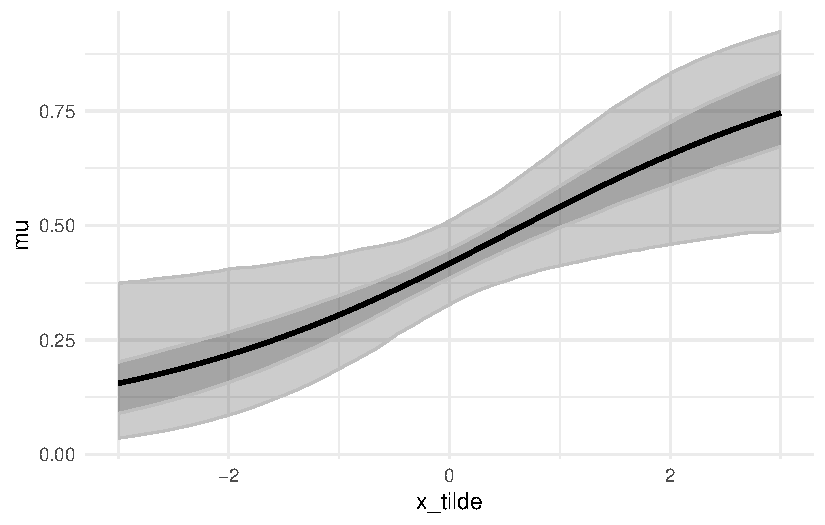
\includegraphics{analysis_files/figure-pdf/unnamed-chunk-9-2.pdf}



\end{document}
